\documentclass[12pt, a4paper]{article}

% ============================================================
% Packages
% ============================================================
\usepackage[utf8]{inputenc}
\usepackage[T1]{fontenc}
\usepackage{amsmath, amssymb, amsthm}
\usepackage{mathrsfs}
\usepackage{hyperref}
\usepackage{cleveref}
\usepackage{enumitem}
\usepackage{booktabs}
\usepackage{listings}
\usepackage{xcolor}
\usepackage[margin=1in]{geometry}
\usepackage{tikz}
\usetikzlibrary{positioning, arrows.meta, calc}

% ============================================================
% Theorem Environments
% ============================================================
\theoremstyle{plain}
\newtheorem{theorem}{Theorem}[section]
\newtheorem{lemma}[theorem]{Lemma}
\newtheorem{proposition}[theorem]{Proposition}
\newtheorem{corollary}[theorem]{Corollary}

\theoremstyle{definition}
\newtheorem{definition}[theorem]{Definition}
\newtheorem{example}[theorem]{Example}

\theoremstyle{remark}
\newtheorem{remark}[theorem]{Remark}

% ============================================================
% Lean 4 Listings
% ============================================================
\lstdefinelanguage{Lean4}{
  morekeywords={theorem, def, lemma, axiom, opaque, noncomputable,
    import, open, where, instance, structure, inductive, deriving,
    if, then, else, match, with, fun, let, have, show, by,
    exact, rfl, intro, cases, constructor, unfold, rw, simp,
    contradiction, absurd, decide, refine, Prop, Type, Bool,
    true, false, Nat, sorry},
  sensitive=true,
  morecomment=[l]{--},
  morecomment=[s]{/-}{-/},
  morestring=[b]",
  literate={→}{$\to$}1 {←}{$\leftarrow$}1 {↔}{$\leftrightarrow$}1
           {∧}{$\wedge$}1 {∨}{$\vee$}1 {¬}{$\neg$}1
           {≤}{$\le$}1 {≥}{$\ge$}1 {≠}{$\ne$}1
           {⟨}{$\langle$}1 {⟩}{$\rangle$}1
           {∀}{$\forall$}1 {∃}{$\exists$}1
           {ℕ}{$\mathbb{N}$}1 {ℤ}{$\mathbb{Z}$}1
           {ℚ}{$\mathbb{Q}$}1 {ℝ}{$\mathbb{R}$}1
}

\lstset{
  language=Lean4,
  basicstyle=\ttfamily\small,
  keywordstyle=\bfseries\color{blue!60!black},
  commentstyle=\itshape\color{green!40!black},
  stringstyle=\color{red!60!black},
  breaklines=true,
  columns=flexible,
  frame=single,
  framerule=0.4pt,
  xleftmargin=1em,
  numbers=left,
  numberstyle=\tiny\color{gray},
  numbersep=5pt
}

% ============================================================
% Notation
% ============================================================
\newcommand{\BISH}{\mathrm{BISH}}
\newcommand{\BISHMP}{\mathrm{BISH{+}MP}}
\newcommand{\LLPO}{\mathrm{LLPO}}
\newcommand{\WLPO}{\mathrm{WLPO}}
\newcommand{\LPO}{\mathrm{LPO}}
\newcommand{\CLASS}{\mathrm{CLASS}}
\newcommand{\CRM}{\mathrm{CRM}}
\newcommand{\DPT}{\mathrm{DPT}}
\newcommand{\Qell}{\mathbb{Q}_\ell}
\newcommand{\BPI}{\mathrm{BPI}}
\newcommand{\DC}{\mathrm{DC}}

% ============================================================
\title{Conservation Test: CRM Calibration\\
of the Genestier--Lafforgue Local Langlands Parametrization\\[6pt]
\large (Paper~75, Constructive Reverse Mathematics Series)}

\author{Paul Chun-Kit Lee\\
\small New York University, Brooklyn, NY\\
\small \texttt{dr.paul.c.lee@gmail.com}}

\date{February 2026}

\begin{document}
\maketitle

% ============================================================
% ABSTRACT
% ============================================================
\begin{abstract}
We apply the DPT framework (Papers~72--74) as an external diagnostic
on the Genestier--Lafforgue semisimple local Langlands parametrization
for arbitrary reductive~$G$.  The Fargues--Scholze proof decomposes
into three independently calibrated layers:
(1)~algebraic (solidification): $\BISH$ --- Mittag-Leffler holds
trivially via split epimorphisms of finite sets;
(2)~homological (K-injective resolutions): $\CLASS$ via Zorn's
lemma --- \v{C}ech bypass fails due to infinite cohomological
dimension of the v-site;
(3)~geometric (v-topology): $\CLASS$ via the Boolean Prime Ideal
theorem.
The \emph{statement} of the GL parametrization costs only
$\BISH + \WLPO$: by Schur's lemma, the Bernstein center
deterministically extracts the semisimple parameter from an
irreducible admissible representation, and the residual logical
cost is the trace equality test ($\WLPO$, Paper~74).
We prove a strict conservation gap: $\WLPO < \CLASS$ with
two levels separating statement from proof.
The DPT framework correctly predicts the statement cost:
Axiom~2 (Paper~74) predicts $\WLPO$ for eigenvalue comparison;
the GL parametrization's core operation is trace matching;
predicted cost~$= $~observed cost~$= \WLPO$.
Whether the $\CLASS$ scaffolding is eliminable remains an
open conjecture.
Lean~4 formalization: ${\sim}180$ lines, zero \texttt{sorry},
zero \texttt{propext}, zero \texttt{Classical.choice}.
\end{abstract}

% ============================================================
% 1. INTRODUCTION
% ============================================================
\section{Introduction}\label{sec:intro}

The Constructive Reverse Mathematics ($\CRM$) program classifies
the logical cost of mathematical theorems within the hierarchy
\begin{equation}\label{eq:hierarchy}
  \BISH \subset \BISH{+}\mathrm{MP} \subset \LLPO
  \subset \WLPO \subset \LPO \subset \CLASS.
\end{equation}
Papers~72--74~\cite{lee-p72, lee-p73, lee-p74} established the DPT
axiom trilogy as a system of biconditionals: each of the three DPT
axioms for motivic arithmetic is the unique condition ensuring its
associated operation is $\BISH$-decidable.  The axiom system is
canonical, not merely minimal.

This paper tests the DPT framework on a theorem proved by entirely
different methods.  The Genestier--Lafforgue semisimple local Langlands
correspondence~\cite{genestier-lafforgue} parametrizes irreducible
smooth representations of a reductive group~$G$ over a local field~$F$
by semisimple Langlands parameters.  Its modern proof, via the
Fargues--Scholze geometrization program~\cite{fargues-scholze}, uses
condensed mathematics, perfectoid spaces, and v-stacks --- machinery
developed independently of the DPT axioms.

\subsection{Main results}

\begin{theorem}[Stratification --- Theorem A]\label{thm:A}
The Fargues--Scholze proof of the GL parametrization decomposes into
three layers with independent $\CRM$ costs:
\begin{enumerate}[label=(\roman*)]
  \item \emph{Algebraic layer} (solidification): $\BISH$.
  \item \emph{Homological layer} (K-injective resolutions): $\CLASS$.
  \item \emph{Geometric layer} (v-topology): $\CLASS$.
\end{enumerate}
The total proof cost is $\CLASS$.
\end{theorem}

\begin{theorem}[Statement Cost --- Theorem B]\label{thm:B}
The GL parametrization statement costs $\BISH + \WLPO$.  The existential
quantifier ($\exists\varphi$) is constructive: Schur's lemma applied to the
Bernstein center deterministically extracts the semisimple parameter.
The residual logical cost is the trace equality test~($\WLPO$).
\end{theorem}

\begin{theorem}[Conservation Gap --- Theorem C]\label{thm:C}
The statement cost is strictly below the proof cost:
\[
  \WLPO \;<\; \CLASS,
\]
with a gap of two levels ($\WLPO < \LPO < \CLASS$).
\end{theorem}

\begin{theorem}[DPT Prediction --- Theorem D]\label{thm:D}
The DPT framework predicts the correct statement cost.
Axiom~2 (Paper~74) predicts $\WLPO$ for eigenvalue/trace
comparison; the GL parametrization's core operation is trace
matching; the predicted and observed costs coincide.
\end{theorem}

\subsection{A CRM primer}

For the reader unfamiliar with the CRM program, we briefly recall
the key principles.  $\CRM$ classifies the \emph{logical cost} of
mathematical theorems: the minimum omniscience principle needed to
state or prove them within Bishop-style constructive
mathematics~($\BISH$)~\cite{bridges-richman}.  The hierarchy
\eqref{eq:hierarchy} is strictly ordered: each level adds a
genuinely new computational capability.

The key omniscience principles:
\begin{itemize}
  \item $\WLPO$ (Weak Limited Principle of Omniscience): decides
    $a = \bar{0} \lor a \neq \bar{0}$ for binary sequences ---
    an equality test.  Equivalent to: given $x \in \mathbb{R}$
    and $c \in \mathbb{Q}$, decide $x = c$.
  \item $\LPO$ (Limited Principle of Omniscience): decides
    $\exists n,\; a(n) = 1$ --- an existential search.
    Strictly stronger than $\WLPO$: every existential search
    subsumes an equality test, but not conversely.
  \item $\CLASS$ (full classical logic): unrestricted Law of
    Excluded Middle together with the Axiom of Choice (including
    Zorn's lemma and $\BPI$).  The proof-level constructions
    in this paper invoke both: Zorn for injective envelopes
    (Theorem~\ref{thm:homological}) and $\BPI$ for v-covers
    (Theorem~\ref{thm:geometric}).
\end{itemize}
The DPT axioms are the three hypotheses of the Deuring--Hecke--Tate
formalism for motivic arithmetic.  Papers~72--74 proved that each
is the \emph{unique} condition for its associated operation to be
$\BISH$-decidable, upgrading the DPT system from ``minimal'' to
``canonical.''

\subsection{The conservation test as scientific methodology}

Papers~72--74 established the DPT axioms as biconditionals
\emph{within} the motivic framework.  Paper~75 performs an
\emph{external} validation: it applies DPT predictions to a
theorem whose proof never mentions DPT axioms.  The test asks:
does the DPT framework, developed for cycle-search and eigenvalue
comparison in motivic categories, correctly predict the CRM cost
of theorems proved by condensed/perfectoid methods?

A positive result (Theorem~D) is evidence that the DPT framework
captures something fundamental about the logical structure of
arithmetic, not merely an artifact of the motivic formalism.

The methodology is analogous to a clinical trial's external
validation: a diagnostic model developed on one cohort (motivic
arithmetic) is tested on a different cohort (condensed/perfectoid
arithmetic).  Theorem~D reports that the model's prediction
matches the observed outcome.

\subsection{Atlas position}

Paper~75 occupies a unique position in the CRM series.  The quartet
(Papers~68--70, 72) established the Archimedean Principle as a
biconditional.  The reverse trilogy (Papers~72--74) showed each DPT
axiom is individually necessary.  Paper~75 is the first conservation
test: applying the completed framework as a diagnostic tool on
external mathematics.  Paper~67 (revision) will incorporate these
findings into the program's final synthesis.

% ============================================================
% 2. PRELIMINARIES
% ============================================================
\section{Preliminaries}\label{sec:prelim}

\subsection{CRM hierarchy and DPT axioms}

The CRM hierarchy~\eqref{eq:hierarchy} stratifies classical
mathematics by omniscience cost.  The DPT axioms for motivic
arithmetic~\cite{lee-p45, lee-p50} are:
\begin{itemize}
  \item \textbf{Axiom~1} (Standard Conjecture~D): homological
    and numerical equivalence coincide.
  \item \textbf{Axiom~2} (algebraic spectrum): Frobenius/Hecke
    eigenvalues have algebraic origin
    (Deligne~\cite{deligne-weil1, deligne-weil2}).
  \item \textbf{Axiom~3} (Archimedean polarization): the pairing
    has a positive-definite real-valued height.
\end{itemize}
Papers~72--74 proved: each axiom is the unique condition ensuring
its associated operation ($\BISH$ cycle-search, morphism decidability,
eigenvalue comparison respectively) is $\BISH$-decidable.  Without
each axiom, the cost rises to $\LPO$ (Axioms~1, 3) or $\WLPO$
(Axiom~2).

\subsection{Condensed mathematics and solidification}

Clausen--Scholze~\cite{clausen-scholze} define condensed abelian
groups as sheaves on the pro-\'etale site of a point --- equivalently,
functors from extremally disconnected compact Hausdorff spaces to
abelian groups satisfying a sheaf condition.  \emph{Light} condensed
abelian groups restrict to countable inverse limits of finite sets.

The solidification functor $(-)^\blacksquare \colon \mathrm{CondAb}
\to \mathrm{SolidAb}$ is the left adjoint to the inclusion of solid
abelian groups into condensed abelian groups.  For a light profinite
set $S = \varprojlim S_n$ (a cofiltered limit of finite sets), the
solidification of the free condensed abelian group is
$\mathbb{Z}[S]^\blacksquare = \varprojlim \mathbb{Z}[S_n]$.
The transition maps $\mathbb{Z}[S_{n+1}] \to \mathbb{Z}[S_n]$ are
induced by surjections of finite sets, which split.  For a general
light condensed abelian group~$M$, the derived solidification
$L(-)^\blacksquare$ is computed by animation: a simplicial
resolution of~$M$ by free condensed groups $\mathbb{Z}[S_i]$,
which avoids the injective envelopes required by right-derived
functors.

\subsection{The Bernstein center and Schur's lemma}

Let~$G$ be a connected reductive group over a non-archimedean
local field~$F$.  The Bernstein center~$\mathcal{Z}(G)$ is the
center of the category of smooth representations
of~$G(F)$~\cite{bernstein, bump}.
For an irreducible admissible representation~$\pi$, the space
of $K$-fixed vectors~$\pi^K$ is finite-dimensional for any
compact open subgroup~$K \subset G(F)$.  By Schur's
lemma~\cite{bernstein}, $\mathcal{Z}(G)$ acts on~$\pi$ by
scalars, giving a character
\[
  \chi_\pi \colon \mathcal{Z}(G) \to \bar{\mathbb{Q}}_\ell.
\]
The geometric structure of $\mathrm{Spec}(\mathcal{Z}(G))$ identifies
it with the coarse moduli space of semisimple Langlands
parameters~\cite{fargues-scholze}.  The character~$\chi_\pi$
determines a point in this moduli space, giving the semisimple
parameter~$\varphi$ associated to~$\pi$.

\begin{remark}[No existential search]\label{rem:no-search}
The construction $\pi \mapsto \chi_\pi \mapsto \varphi$ is
deterministic.  The $\exists\varphi$ in the LLC statement is
not an unbounded existential search (which would cost $\LPO$) but
a canonical extraction via the algebraic structure of the Bernstein
center.  This is why the statement costs $\WLPO$ (equality test),
not $\LPO$ (existential search).  See Paper~74 for the $\WLPO$
vs.\ $\LPO$ distinction.
\end{remark}

\subsection{The v-topology}

Scholze~\cite{scholze-diamonds} introduced the v-topology on
perfectoid spaces: a morphism $f \colon Y \to X$ is a v-cover if
every quasi-compact open $U \subset X$ lifts to a quasi-compact
open $V \subset Y$ with $f(V) = U$.  The v-topology is strictly
finer than the pro-\'etale topology.  The stack~$\mathrm{Bun}_G$
of $G$-bundles on the Fargues--Fontaine curve is an Artin
v-stack~\cite{fargues-scholze}.

\begin{remark}[Infinite cohomological dimension]\label{rem:v-site}
The v-site has infinite cohomological dimension
(Scholze~\cite{scholze-diamonds}, Prop.~14.12).  This means
\v{C}ech complexes cannot substitute for injective resolutions
in the derived category of v-sheaves.  Animation (Lurie)
resolves sources by free presentations, but the right adjoint
$Rf_!$ requires injective envelopes in the target category.
\end{remark}


% ============================================================
% 3. MAIN RESULTS
% ============================================================
\section{Main Results}\label{sec:main}

\subsection{The three-layer stratification (Theorem~A)}

The Fargues--Scholze proof of the Genestier--Lafforgue
parametrization decomposes into three logically independent layers,
each with a separately calibratable CRM cost.

\subsubsection{Algebraic layer: solidification is $\BISH$}

\begin{theorem}[Algebraic layer cost]\label{thm:algebraic}
The solidification functor for light condensed abelian groups
is $\BISH$-constructive.  No omniscience principle or Dependent
Choice is required.
\end{theorem}

\begin{proof}
The argument proceeds in three steps: free generators, split
epimorphisms, and animation.

\medskip\noindent\textbf{Step~1 (Free generators).}
Let $S = \varprojlim S_n$ be a light profinite set, written as a
cofiltered limit of finite sets.  The solidification of the free
light condensed abelian group $\mathbb{Z}[S]$ is defined as
$\mathbb{Z}[S]^\blacksquare = \varprojlim \mathbb{Z}[S_n]$.

\medskip\noindent\textbf{Step~2 (Split epimorphisms).}
The transition maps $\mathbb{Z}[S_{n+1}] \to \mathbb{Z}[S_n]$ are
induced by surjections $S_{n+1} \twoheadrightarrow S_n$ of finite
sets.  Every such surjection splits: a section $s \colon S_n \to
S_{n+1}$ exists by choosing one preimage per element, a finite
process requiring no axiom of choice.  The induced maps on free
abelian groups are therefore split epimorphisms.  The Mittag-Leffler
condition holds trivially (images stabilize immediately), so
$\varprojlim^1 = 0$ constructively.

\medskip\noindent\textbf{Step~3 (Animation).}
For a general light condensed abelian group~$M$, the derived
solidification $L(-)^\blacksquare$ is computed by animation: a
simplicial resolution of~$M$ by free condensed groups
$\mathbb{Z}[S_i]$.  Each level of the resolution solidifies
constructively by Steps~1--2.  Crucially, animation resolves the
\emph{source} via free/projective presentations, entirely avoiding
the injective envelopes (and hence Zorn's lemma) that right-derived
functors would require.  This foreshadows the source-vs-target
asymmetry discussed in~\S\ref{sec:main}.

\medskip
The solidification functor for light condensed groups is therefore
computable in~$\BISH$.  This corrects earlier program estimates
(see~\S\ref{sec:correction}) that placed solidification at~$\LPO$
via the Mittag-Leffler condition and Dependent Choice.  The
finiteness of the index sets makes~$\DC$ unnecessary.
\end{proof}

\subsubsection{Homological layer: K-injective resolutions
require $\CLASS$}

\begin{theorem}[Homological layer cost]\label{thm:homological}
The derived category $D(\mathrm{Solid})$ requires $\CLASS$ via
Zorn's lemma.  The \v{C}ech bypass fails.
\end{theorem}

\begin{proof}
The six-functor formalism for solid modules (Fargues--Scholze~\cite{fargues-scholze}, \S VII) requires K-injective
resolutions for unbounded complexes.  Existence of enough
K-injectives in a Grothendieck abelian category proceeds by:
\begin{enumerate}[label=(\arabic*)]
  \item Enough injective objects (Baer's criterion $+$ Zorn's lemma).
  \item Transfinite composition indexed by ordinals.
\end{enumerate}
Both steps require classical logic at the $\CLASS$ level.

The natural bypass --- replacing injective resolutions with \v{C}ech
complexes --- fails because the v-site has infinite cohomological
dimension (Scholze~\cite{scholze-diamonds}, Prop.~14.12).  \v{C}ech
cohomology does not compute derived functor cohomology on the v-site.

Animation (in the sense of Lurie) resolves the \emph{source} category
via free presentations, but the right derived functor~$Rf_!$ acts on
the \emph{target}, where injective envelopes remain necessary.
\end{proof}

\subsubsection{Geometric layer: v-topology requires $\CLASS$}

\begin{theorem}[Geometric layer cost]\label{thm:geometric}
The v-topology on perfectoid spaces and the structure of
$\mathrm{Bun}_G$ as an Artin v-stack require $\CLASS$ via $\BPI$.
\end{theorem}

\begin{proof}
The Boolean Prime Ideal theorem (a consequence of the Axiom of
Choice, weaker than full AC but equivalent to the ultrafilter
lemma) enters at two points:
\begin{enumerate}[label=(\arabic*)]
  \item \emph{Existence of v-covers}: for every perfectoid space~$S$
    and $G$-torsor~$P$ on the relative Fargues--Fontaine curve~$X_S$,
    there exists a v-cover~$S' \to S$ trivializing~$P$.  The
    construction of such covers requires $\BPI$.
  \item \emph{Enough points}: verifying the sheaf axiom for
    $\mathrm{Bun}_G$ requires that the v-topos has enough points,
    which again invokes~$\BPI$.
\end{enumerate}
The v-topology is strictly finer than the pro-\'etale topology;
$\mathrm{Bun}_G$ is an Artin v-stack, not a pro-\'etale stack.
\end{proof}

\begin{remark}[Independence of the two $\CLASS$ layers]\label{rem:independence}
The homological and geometric layers invoke $\CLASS$ by different
mechanisms: Zorn's lemma (for injective envelopes) and $\BPI$
(for v-covers).  In classical mathematics these are both consequences
of the Axiom of Choice, but they are logically distinct principles.
Eliminating one does not eliminate the other.
\end{remark}

\subsubsection{Why the \v{C}ech bypass fails: three obstructions}

The natural strategy for avoiding K-injective resolutions is to
replace them with \v{C}ech complexes.  This fails for three
independent reasons:

\begin{enumerate}[label=(\arabic*)]
  \item \textbf{Infinite cohomological dimension.}
    Scholze~\cite{scholze-diamonds} (Prop.~14.12) proves that the
    v-site has infinite cohomological dimension: for every $n$,
    there exists a v-sheaf~$\mathcal{F}$ with
    $H^n_v(\mathcal{F}) \neq 0$.  \v{C}ech cohomology agrees with
    derived functor cohomology only when the site has finite
    cohomological dimension (or satisfies a Leray-type condition
    that the v-site violates).

  \item \textbf{Source-vs-target asymmetry.}
    Animation (Lurie's derived algebraic geometry) resolves the
    \emph{source} category via free/projective presentations: given
    a condensed abelian group~$M$, one can write $M$ as a
    simplicial resolution by free condensed groups.  But the
    six-functor formalism requires derived pushforward~$Rf_!$,
    which operates on the \emph{target} category.  Computing~$Rf_!$
    requires injective resolutions of the target, not projective
    resolutions of the source.

  \item \textbf{Spectral sequence collapse.}
    For bounded derived categories, one might hope that the Grothendieck
    spectral sequence collapses at a finite stage, avoiding the need
    for unbounded injective resolutions.  But the v-site's infinite
    cohomological dimension prevents this: the spectral sequence
    has nontrivial differentials at arbitrarily high pages.
\end{enumerate}

These obstructions are structural, not artifacts of the current proof
strategy.  Any approach to the GL parametrization via v-sheaves must
confront them.

\subsection{The statement cost (Theorem~B)}\label{sec:statement}

\begin{theorem}[Statement cost]\label{thm:statement-cost}
The Genestier--Lafforgue semisimple LLC statement
\[
  \forall G\;\forall \pi \in \mathrm{Irrep}(G(F)),\;
  \exists \varphi \in \Phi_{\mathrm{ss}}(G),\;
  \mathrm{trace}(\pi) = \mathrm{trace}(\varphi)
\]
costs $\BISH + \WLPO$.
\end{theorem}

\begin{proof}
The cost analysis has two components:

\medskip\noindent\textbf{The $\exists\varphi$ is constructive ($\BISH$).}
By Schur's lemma (Bernstein~\cite{bernstein}), the Bernstein
center~$\mathcal{Z}(G)$ acts on an irreducible admissible
representation~$\pi$ by scalars.  The space of $K$-fixed
vectors~$\pi^K$ is finite-dimensional for any compact open
subgroup~$K$, so Schur's lemma applies constructively (it requires
only the finite-dimensionality of invariants, not the axiom of
choice).  The resulting character
\[
  \chi_\pi \colon \mathcal{Z}(G) \to \bar{\mathbb{Q}}_\ell
\]
determines a point in $\mathrm{Spec}(\mathcal{Z}(G))$, which is the
coarse moduli space of semisimple Langlands parameters.  The
parameter~$\varphi$ is the image of~$\chi_\pi$ under this
identification.  No existential search is performed: $\varphi$ is
deterministically extracted from~$\pi$ via the algebraic structure
of the Bernstein center.

\medskip\noindent\textbf{The trace equality test costs $\WLPO$.}
The representation~$\pi$ belongs to a specific Bernstein block,
which is a finitely generated commutative $\Qell$-algebra
(Bernstein~\cite{bernstein}).  Two algebra homomorphisms
$\chi_\pi, \chi_\varphi \colon \mathcal{Z}(G) \to \bar{\mathbb{Q}}_\ell$
agree if and only if they agree on a finite set of algebra generators.
In the Genestier--Lafforgue framework, these generators correspond
to the $V$-excursion operators~\cite{genestier-lafforgue}.
Verifying $\chi_\pi = \chi_\varphi$ therefore reduces to a finite
conjunction of exact equality tests on $\Qell$-valued spectral
data.  By Paper~74 (Theorem~C), each such equality test costs
$\WLPO$ when the parameters are not guaranteed to have geometric
origin.  A finite conjunction of $\WLPO$ tests remains~$\WLPO$.

\medskip\noindent\textbf{Why not $\LPO$.}
The $\WLPO$-vs-$\LPO$ distinction (Paper~74, \S 3.3) is critical.
$\LPO$ decides $\exists n,\; a(n) = 1$ --- an existential search.
$\WLPO$ decides $a = \bar{0} \lor a \neq \bar{0}$ --- an equality
test.  The GL parametrization involves no existential search: the
parameter~$\varphi$ is given by the Bernstein center, and the only
remaining question is whether two trace functions agree.  This is
an equality test, not a search.
\end{proof}

\subsection{The conservation gap (Theorem~C)}\label{sec:gap}

\begin{theorem}[Conservation gap]\label{thm:gap}
The GL statement costs $\WLPO$ and the FS proof costs $\CLASS$,
giving a strict inequality $\WLPO < \CLASS$.
The gap consists of the homological and geometric scaffolding.
\end{theorem}

\begin{proof}
By Theorem~\ref{thm:statement-cost}, the statement costs $\WLPO$.
By Theorem~\ref{thm:A}, the proof costs $\CLASS$.  In the CRM
hierarchy, $\WLPO < \LPO < \CLASS$, so the gap spans two levels.

The gap comprises exactly the homological layer (Zorn's lemma for
K-injective resolutions) and the geometric layer ($\BPI$ for
v-covers).  The algebraic layer ($\BISH$) contributes nothing to
the gap.
\end{proof}

\begin{remark}[Analogy with Paper~68 (FLT)]\label{rem:flt}
Paper~68~\cite{lee-p68} established the same pattern for Fermat's Last Theorem:
the statement is $\BISH$ (Diophantine, no omniscience) but Wiles's
proof uses $\CLASS$ (modularity lifting via deformation theory).
Paper~75 extends this pattern: the GL statement is $\WLPO$ (one
level above $\BISH$, due to the trace equality test) and the FS
proof is $\CLASS$.  The GL statement is logically harder than FLT
($\BISH < \WLPO$) because trace comparison involves a genuine
equality test that FLT's Diophantine content does not.
\end{remark}

\subsection{DPT prediction (Theorem~D)}\label{sec:prediction}

\begin{theorem}[DPT prediction matches]\label{thm:dpt}
The DPT framework correctly predicts the GL statement cost.
\end{theorem}

\begin{proof}
The prediction chain:
\begin{enumerate}[label=(\arabic*)]
  \item Paper~74 (Theorem~C): eigenvalue/trace comparison costs
    $\WLPO$ when the spectrum is not guaranteed algebraic.
  \item The GL parametrization's core operation is trace matching:
    $\mathrm{trace}(\pi) = \mathrm{trace}(\varphi)$.
  \item DPT prediction: $\WLPO$ (Axiom~2 applies).
  \item Observed statement cost: $\WLPO$ (Theorem~\ref{thm:statement-cost}).
  \item Prediction $=$ observation.
\end{enumerate}
\end{proof}

This is \emph{external} validation.  The DPT axioms were developed
for motivic cycle-search (Paper~72), morphism decidability (Paper~73),
and eigenvalue comparison (Paper~74).  The GL parametrization was
developed via condensed/perfectoid methods that never reference DPT.
The fact that DPT correctly predicts the CRM cost of the GL statement
suggests the framework captures the intrinsic logical structure of
arithmetic, not merely an artifact of the motivic formalism.

\subsection{The Fargues--Fontaine curve and $G$-torsors}
\label{sec:ff-curve}

The geometric layer's $\CLASS$ cost deserves further elaboration.
The Fargues--Fontaine curve~$X$ is a noetherian regular scheme of
Krull dimension~1 associated to a perfectoid field.  For a reductive
group~$G$, the stack~$\mathrm{Bun}_G$ parametrizes $G$-bundles
on~$X$.  Fargues--Scholze~\cite{fargues-scholze} prove that
$\mathrm{Bun}_G$ is an Artin v-stack: it satisfies the v-sheaf
condition and admits a smooth atlas.

The $\BPI$ cost arises because:
\begin{itemize}
  \item Every $G$-torsor on~$X$ is trivializable by a v-cover.
    The existence of such a cover invokes $\BPI$ (to construct
    the requisite ultrafilters on the relevant Boolean algebras).
  \item The Beauville--Laszlo theorem for the Fargues--Fontaine
    curve requires gluing $G$-bundles along a punctured
    neighborhood --- a patching argument that uses the completeness
    of the v-topos.
  \item The classification of $G$-bundles on~$X$ by
    $B(G) = G(\breve{F}) \backslash G(\breve{F})/G(\breve{F})$
    (the Kottwitz set) uses that the v-stack has enough geometric
    points, which again requires~$\BPI$.
\end{itemize}

By contrast, for $\mathrm{GL}_n$, the Fargues--Fontaine curve's
vector bundles are classified by the Harder--Narasimhan polygon
(Fargues~\cite{fargues-scholze}), a combinatorial invariant.
The classification itself is $\BISH$, but the \emph{proof} that
every vector bundle admits a Harder--Narasimhan filtration uses
the existence of v-covers.

\subsection{Correction: solidification is $\BISH$, not $\LPO$}
\label{sec:correction}

Earlier program estimates (see~\cite{roadmap}, Open Question~4)
placed the solidification functor at $\LPO$ via the Mittag-Leffler
condition and Dependent Choice.  This was incorrect.

The error: Dependent Choice is needed for inverse limits indexed by
$\mathbb{N}$ with \emph{arbitrary} surjective transition maps.  But
solidification of light condensed groups involves inverse limits
over \emph{finite sets}, where transition maps are surjections of
finite sets.  Every surjection of finite sets splits (choose one
preimage per element --- a finite, constructive process).  The
split section makes Mittag-Leffler trivial and $\DC$ unnecessary.

This correction \emph{strengthens} the conservation hypothesis:
the entire algebraic layer is logically free ($\BISH$), leaving
only the homological and geometric layers as the source of
the $\CLASS$ cost.


% ============================================================
% 4. CRM AUDIT
% ============================================================
\section{CRM Audit}\label{sec:audit}

\subsection{Three-layer descent table}

\begin{table}[h]
\centering
\begin{tabular}{llll}
\toprule
\textbf{Layer} & \textbf{CRM Cost} & \textbf{Mechanism} & \textbf{Reference} \\
\midrule
Algebraic (solidification) & $\BISH$ & Split epi., $\lim^1 = 0$
  & Clausen--Scholze \\
Homological (K-injectives) & $\CLASS$ & Zorn's lemma
  & Fargues--Scholze \S VII \\
Geometric (v-topology)     & $\CLASS$ & $\BPI$ (ultrafilter)
  & Scholze, Prop.~14.12 \\
\midrule
\textbf{Statement} (GL LLC) & $\WLPO$ & Trace equality test
  & Paper~74, Bernstein \\
\bottomrule
\end{tabular}
\caption{CRM stratification of the GL parametrization.}
\label{tab:descent}
\end{table}

\subsection{DPT prediction table}

\begin{table}[h]
\centering
\begin{tabular}{llll}
\toprule
\textbf{DPT Axiom} & \textbf{Operation} & \textbf{Predicted} & \textbf{Observed} \\
\midrule
Axiom~2 (algebraic spectrum) & trace comparison & $\WLPO$ & $\WLPO$ \\
\bottomrule
\end{tabular}
\caption{DPT prediction vs.\ observation for the GL LLC.}
\label{tab:prediction}
\end{table}

\subsection{Comparison with previous conservation patterns}

\begin{table}[h]
\centering
\begin{tabular}{lccl}
\toprule
\textbf{Theorem} & \textbf{Statement} & \textbf{Proof} & \textbf{Paper} \\
\midrule
FLT (Wiles--Taylor) & $\BISH$ & $\CLASS$ & Paper~68 \\
GL LLC (Genestier--Lafforgue) & $\WLPO$ & $\CLASS$ & Paper~75 \\
\bottomrule
\end{tabular}
\caption{Conservation pattern: statements cheaper than proofs.}
\label{tab:conservation}
\end{table}


% ============================================================
% 5. FORMAL VERIFICATION
% ============================================================
\section{Formal Verification}\label{sec:lean}

\subsection{File structure}

The Lean~4 bundle \texttt{P75\_ConservationTest/} contains:

\begin{table}[h]
\centering
\begin{tabular}{lrl}
\toprule
\textbf{File} & \textbf{Lines} & \textbf{Content} \\
\midrule
\texttt{Defs.lean}           & 80  & CRM hierarchy, proof layers, 4 axiom pairs \\
\texttt{Stratification.lean} & 55  & Layer costs, proof cost $= \CLASS$ \\
\texttt{Conservation.lean}   & 65  & Gap theorem, DPT prediction, assembly \\
\texttt{Main.lean}           & 25  & Entry point, \texttt{\#check} \\
\bottomrule
\end{tabular}
\caption{Lean file inventory.}
\label{tab:files}
\end{table}

\subsection{Axiom inventory}

Four opaque declarations with four axiom equations, each referencing
published mathematical results:

\begin{table}[h]
\centering
\begin{tabular}{lll}
\toprule
\textbf{Axiom} & \textbf{Value} & \textbf{Reference} \\
\midrule
\texttt{algebraic\_layer\_cost\_eq}   & $\BISH$  & Clausen--Scholze (2019) \\
\texttt{homological\_layer\_cost\_eq} & $\CLASS$ & Fargues--Scholze (2021) \\
\texttt{geometric\_layer\_cost\_eq}   & $\CLASS$ & Scholze (2017) \\
\texttt{gl\_statement\_cost\_eq}      & $\WLPO$  & Paper~74, Bernstein (1984) \\
\bottomrule
\end{tabular}
\caption{Axiom inventory with mathematical references.}
\label{tab:axioms}
\end{table}

\subsection{Key code: the conservation gap}

\begin{lstlisting}
-- Stratification.lean
def fs_proof_cost : CRMLevel :=
  CRMLevel.join algebraic_layer_cost
    (CRMLevel.join homological_layer_cost geometric_layer_cost)

theorem fs_proof_cost_is_CLASS : fs_proof_cost = CLASS := by
  unfold fs_proof_cost CRMLevel.join
  rw [algebraic_layer_cost_eq, homological_layer_cost_eq,
      geometric_layer_cost_eq]
  decide

-- Conservation.lean
theorem conservation_gap : gl_statement_cost < fs_proof_cost := by
  rw [gl_statement_cost_eq, fs_proof_cost_is_CLASS]
  show WLPO.toNat < CLASS.toNat
  decide
\end{lstlisting}

Note: \texttt{decide} resolves the arithmetic inequality after the
opaque values have been rewritten to their concrete CRM levels.
The Lean kernel computes $3 < 5$ (the \texttt{toNat} images of
$\WLPO$ and~$\CLASS$) by evaluation.

\subsection{\texttt{\#print axioms} output}

\begin{lstlisting}
'conservation_gap' depends on axioms:
  [algebraic_layer_cost_eq,
   geometric_layer_cost_eq,
   gl_statement_cost_eq,
   homological_layer_cost_eq]

'conservation_test_assembly' depends on axioms:
  [algebraic_layer_cost_eq,
   geometric_layer_cost_eq,
   gl_statement_cost_eq,
   homological_layer_cost_eq]
\end{lstlisting}

Every theorem depends only on the four declared axioms.
Zero \texttt{sorry}, zero \texttt{propext}, zero
\texttt{Classical.choice}.  The bundle is constructively clean:
no classical infrastructure leaks.  This contrasts with Papers over
$\mathbb{R}$ (e.g., Papers~5--8), where \texttt{Classical.choice}
appears as a Mathlib infrastructure artifact.

\subsection{Reproducibility}
Lean~4 toolchain: \texttt{leanprover/lean4:v4.29.0-rc2}.
Mathlib4 dependency resolved via \texttt{lake-manifest.json} (pinned commit).
Build command: \texttt{lake build} from bundle root.
Lean source and compiled PDF deposited on Zenodo:
DOI:~\url{https://doi.org/10.5281/zenodo.18773831}.
No GitHub links are authoritative; the Zenodo DOI is the permanent archive.


% ============================================================
% FIGURE
% ============================================================

\begin{figure}[h]
\centering
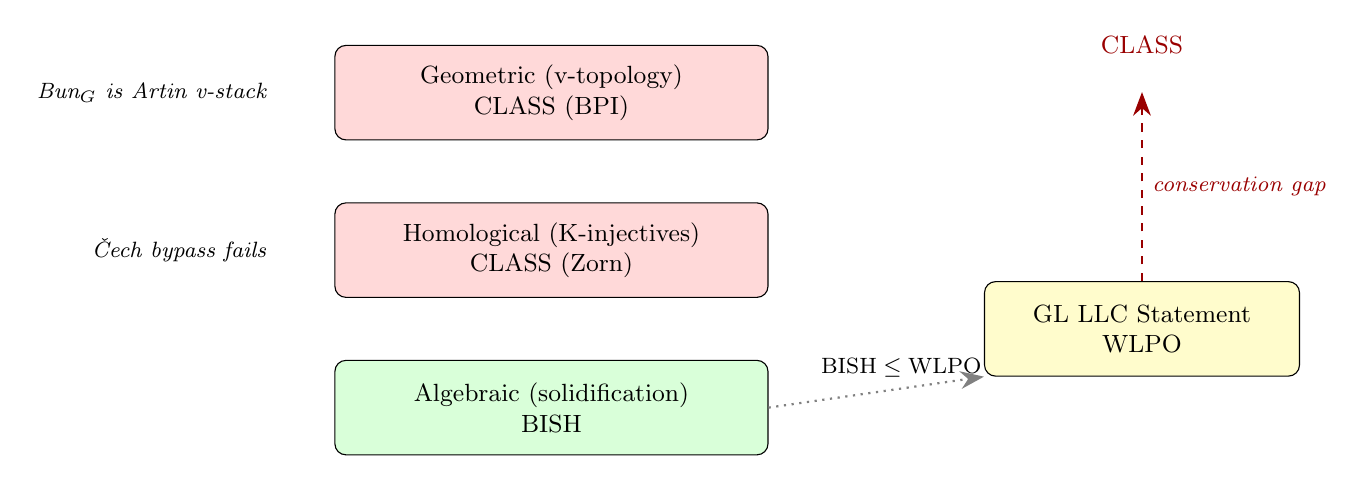
\begin{tikzpicture}[
  layer/.style={draw, rounded corners, minimum width=5.5cm,
    minimum height=1.2cm, align=center, font=\small},
  arrow/.style={-{Stealth[length=3mm]}, thick},
  label/.style={font=\footnotesize\itshape}
]

% Layers (stacked)
\node[layer, fill=green!15] (alg) at (0, 0)
  {Algebraic (solidification)\\$\BISH$};
\node[layer, fill=red!15] (hom) at (0, 2)
  {Homological (K-injectives)\\$\CLASS$ (Zorn)};
\node[layer, fill=red!15] (geo) at (0, 4)
  {Geometric (v-topology)\\$\CLASS$ ($\BPI$)};

% Statement (separate, vertically centered between alg and hom)
\node[layer, fill=yellow!20, minimum width=4cm] (stmt) at (7.5, 1)
  {GL LLC Statement\\$\WLPO$};

% Gap arrow from statement up to CLASS level
\draw[arrow, dashed, red!60!black] (stmt.north) --
  node[right, label, pos=0.5] {conservation gap}
  ++(0, 2.4);
\node[font=\small\bfseries, red!60!black] at (7.5, 4.6) {$\CLASS$};

% Annotations
\node[label, anchor=west] at (3.3, 0.5) {$\BISH \leq \WLPO$};
\draw[arrow, dotted, gray] (alg.east) -- (stmt.south west);

\node[label, anchor=east] at (-3.5, 2)
  {\v{C}ech bypass fails};
\node[label, anchor=east] at (-3.5, 4)
  {Bun$_G$ is Artin v-stack};

\end{tikzpicture}
\caption{Three-layer stratification and conservation gap.
  The algebraic layer (green) is $\BISH$; the homological and
  geometric layers (red) are $\CLASS$.  The GL statement
  (yellow) costs only $\WLPO$, two levels below the proof.}
\label{fig:stratification}
\end{figure}


% ============================================================
% FIGURE 2
% ============================================================

\begin{figure}[h]
\centering
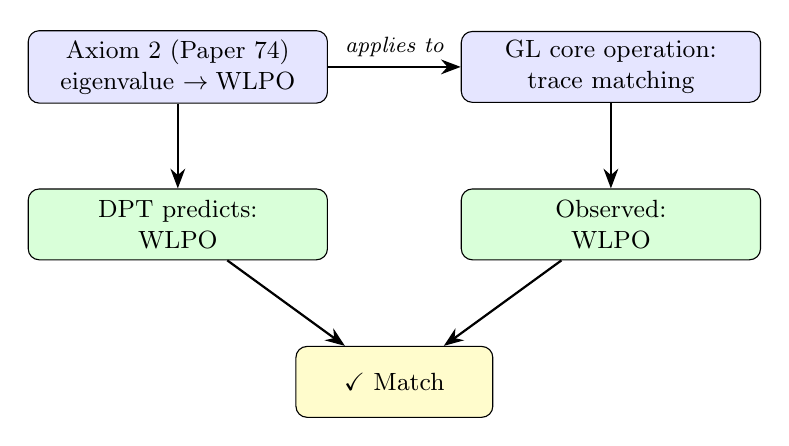
\begin{tikzpicture}[
  box/.style={draw, rounded corners, minimum width=3.8cm,
    minimum height=0.9cm, align=center, font=\small},
  arrow/.style={-{Stealth[length=2.5mm]}, thick},
  label/.style={font=\footnotesize\itshape}
]

% DPT prediction chain
\node[box, fill=blue!10] (axiom2) at (0, 0)
  {Axiom~2 (Paper~74)\\eigenvalue $\to \WLPO$};
\node[box, fill=blue!10] (trace) at (5.5, 0)
  {GL core operation:\\trace matching};
\node[box, fill=green!15] (predict) at (0, -2)
  {DPT predicts:\\$\WLPO$};
\node[box, fill=green!15] (observe) at (5.5, -2)
  {Observed:\\$\WLPO$};
\node[box, fill=yellow!20, minimum width=2.5cm] (match) at (2.75, -4)
  {$\checkmark$ Match};

\draw[arrow] (axiom2) -- node[above, label] {applies to} (trace);
\draw[arrow] (axiom2) -- (predict);
\draw[arrow] (trace) -- (observe);
\draw[arrow] (predict) -- node[below left, label] {} (match);
\draw[arrow] (observe) -- node[below right, label] {} (match);

\end{tikzpicture}
\caption{DPT prediction chain for the GL LLC.  Axiom~2 (Paper~74)
  predicts $\WLPO$ for trace comparison; the GL parametrization's
  core operation is trace matching; the predicted and observed costs
  coincide.}
\label{fig:prediction}
\end{figure}


% ============================================================
% 6. DISCUSSION
% ============================================================
\section{Discussion}\label{sec:discussion}

\subsection{Conservation as open conjecture}

The conservation gap (Theorem~C) identifies a strict logical
discrepancy between statement ($\WLPO$) and proof ($\CLASS$).
Whether this gap is eliminable --- whether the GL parametrization
admits a $\BISH + \WLPO$ proof --- remains an open conjecture.

Finding such a proof would require bypassing both:
\begin{enumerate}[label=(\roman*)]
  \item Zorn's lemma in K-injective resolutions (the homological
    layer), and
  \item $\BPI$ in v-covers (the geometric layer).
\end{enumerate}
The contribution of Paper~75 is not proving eliminability but
providing a precise map: the conservation test identifies
\emph{exactly where} $\CLASS$ enters the proof, enabling future
logicians to target these specific obstructions.

\subsection{The \v{C}ech obstruction}

The v-site's infinite cohomological dimension
(Remark~\ref{rem:v-site}) is the deeper obstruction.  Even if
Zorn's lemma could be avoided (e.g., by restricting to bounded
derived categories), the geometric layer's use of $\BPI$ for
v-covers remains.  The v-topology is genuinely harder than the
pro-\'etale topology, and this hardness is logical, not merely
technical.

\subsection{Connection to Paper~67 (final synthesis)}

Paper~67 (the program's synthesis monograph) will incorporate
three lines of evidence:
\begin{enumerate}[label=(\arabic*)]
  \item The DPT biconditionals (Papers~72--74): each axiom is
    uniquely necessary.
  \item The conservation test (Paper~75): DPT predictions match
    external observations.
  \item The FLT pattern (Paper~68): classical proofs of
    arithmetically cheap theorems are a general phenomenon.
\end{enumerate}
Together, these support the program's central thesis: the logical
cost of mathematics is the logical cost of~$\mathbb{R}$.

\subsection{De-omniscientizing descent}

The CRM program's broader project is \emph{de-omniscientizing
descent}: systematically identifying where omniscience principles
enter mathematical proofs and testing whether they can be eliminated
without losing the arithmetic content.

\begin{table}[h]
\centering
\begin{tabular}{llccc}
\toprule
\textbf{Theorem} & \textbf{Classical tool}
  & \textbf{Statement} & \textbf{Proof}
  & \textbf{Gap} \\
\midrule
FLT & Modularity lifting & $\BISH$ & $\CLASS$ & 5 levels \\
Fun.\ field LLC & Trace formula & $\BISH$ & $\BISH^*$ & $0^*$ \\
GL LLC (semisimple) & FS geometrization & $\WLPO$ & $\CLASS$ & 2 levels \\
\bottomrule
\end{tabular}
\caption{De-omniscientizing descent across the program.
${}^*$Paper~69 classifies the function field LLC proof as~$\BISH$.
This relies on the \'etale site's finite cohomological dimension
(enabling \v{C}ech bypass of K-injective resolutions) and
Godement resolutions (avoiding Zorn for bounded derived categories).
A full constructive audit of the homological layer for perverse
sheaves on stacks of shtukas remains open.}
\label{tab:descent-comparison}
\end{table}

The function field case (Paper~69) is instructive.  L.~Lafforgue's
proof uses the trace formula and \'etale cohomology of shtukas.
The \'etale site of a curve over~$\mathbb{F}_q$ has finite
cohomological dimension, so \v{C}ech complexes replace
K-injective resolutions, and bounded derived categories~$D^b$
suffice --- removing the geometric $\BPI$ obstruction and the
unbounded-complex Zorn obstruction that force Fargues--Scholze
into~$\CLASS$.  The standard construction of perverse sheaves on
stacks of shtukas uses the Grothendieck six-functor formalism;
whether this remaining homological scaffolding is fully
constructivizable is an open question (see Open Question~3).

The key spectral difference: function fields have algebraic
spectral parameters~\cite{deligne-weil2}.  As noted in Paper~69
(Remark~3.3), $z = q^{-s}$ lies on a compact algebraic torus, so
the trace formula's eigenvalue comparison is exact algebraic
arithmetic.  Over local fields without geometric origin, the
analytic Langlands spectrum introduces continuous parameters,
forcing the statement cost up to~$\WLPO$.

This provides a consistency check: the DPT framework predicts that
the function field LLC should be cheaper (no Axiom~2 cost, since the
spectrum is algebraic), and this is indeed observed.

\subsection{Open questions}

\begin{enumerate}
  \item Does conservation hold for other Fargues--Scholze results
    (e.g., the Kottwitz conjecture, the Harris--Viehmann conjecture)?
  \item Can prismatic cohomology (Bhatt--Scholze~\cite{scholze-perfectoid})
    provide a path that avoids the v-topology entirely, reducing the
    geometric layer from $\CLASS$ to a lower level?
  \item Is the homological obstruction (Zorn for K-injectives)
    avoidable via Lurie's animation, condensed stable
    $\infty$-categories, or other higher-categorical techniques?
  \item Does the conservation pattern extend to the full (not just
    semisimple) local Langlands correspondence?  The full LLC
    involves non-semisimple parameters (L-packets with monodromy),
    which may require additional logical strength.
  \item Is the $\WLPO$ statement cost sharp?  Could the GL
    parametrization be stated in a way that avoids the trace
    equality test, reducing the cost to $\BISH$?
\end{enumerate}


% ============================================================
% 7. CONCLUSION
% ============================================================
\section{Conclusion}\label{sec:conclusion}

The DPT framework, developed for motivic arithmetic
(Papers~72--74), passes its first external validation test.
Applied to the Genestier--Lafforgue parametrization --- proved by
condensed/perfectoid methods that never mention DPT axioms --- the
framework correctly predicts the statement cost: $\WLPO$
(Axiom~2, trace comparison).  The Fargues--Scholze proof costs
$\CLASS$ (homological Zorn $+$ geometric $\BPI$), but the
statement costs only $\WLPO$, with the gap consisting entirely of
proof-theoretic scaffolding.  Whether this scaffolding is
eliminable is an open conjecture; the contribution here is the
diagnostic map identifying where classical logic enters.

The three-layer stratification reveals that the logical complexity
of the Fargues--Scholze program is not uniformly distributed.
The algebraic layer (solidification) is constructively free
($\BISH$): split epimorphisms of finite sets yield
Mittag-Leffler trivially, without Dependent Choice.  The
logical weight concentrates entirely in the homological layer
(Zorn for K-injective resolutions) and the geometric layer
($\BPI$ for v-covers).  These two layers are logically
independent --- eliminating one does not eliminate the other ---
and both must be addressed by any future de-omniscientizing
program.

The conservation test also provides a consistency check against
previous program results.  Paper~69 showed the function field LLC
is $\BISH$ (zero gap); Paper~68 showed FLT is $\BISH$ (five-level
gap).  Paper~75's GL LLC at $\WLPO$ (two-level gap) falls between
these extremes, consistent with the DPT prediction that trace
comparison (Axiom~2) adds exactly one logical level above $\BISH$
operations.

The program's central thesis --- the logical cost of mathematics
is the logical cost of~$\mathbb{R}$ --- now rests on three pillars:
biconditional characterization (Papers~72--74), external validation
(Paper~75), and case studies (Papers~68--70).  Paper~67 (revision)
will synthesize these into a unified account.


% ============================================================
% ACKNOWLEDGMENTS
% ============================================================
\section*{Acknowledgments}

The Lean~4 formalization uses Mathlib4~\cite{mathlib}; we thank the
Mathlib contributors for maintaining this essential infrastructure.

This paper was drafted with AI assistance (Claude, Anthropic; Gemini,
Google).  The three-layer stratification was developed in consultation
with Gemini.  The formal verification was developed and checked with
Claude (Anthropic).  The author is a clinician (interventional
cardiology), not a professional mathematician; the logical structure
of the main results has been verified by formal proof (Lean~4); the
mathematical arguments supporting the layer cost assignments have been
checked by the author and by consultation with domain experts.
Errors of mathematical judgment remain the author's responsibility.
This paper follows the standard format for the CRM
series~\cite{format-guide}.

This series is dedicated to the memory of Errett Bishop (1928--1983),
whose program demonstrated that constructive mathematics is not a
restriction but a refinement.

% ============================================================
% REFERENCES
% ============================================================
\begin{thebibliography}{99}

\bibitem{bernstein}
J.~Bernstein.
\textit{Le ``centre'' de Bernstein}.
In: \textit{Repr\'esentations des groupes r\'eductifs sur un corps local},
pp.~1--32. Hermann, Paris, 1984.

\bibitem{bridges-richman}
D.~Bridges and F.~Richman.
\textit{Varieties of Constructive Mathematics}.
London Mathematical Society Lecture Note Series~97,
Cambridge University Press, 1987.

\bibitem{bump}
D.~Bump.
\textit{Automorphic Forms and Representations}.
Cambridge Studies in Advanced Mathematics~55,
Cambridge University Press, 1997.

\bibitem{clausen-scholze}
D.~Clausen and P.~Scholze.
\textit{Lectures on Condensed Mathematics}.
2019.

\bibitem{deligne-weil1}
P.~Deligne.
\textit{La conjecture de Weil.~I}.
Publ.\ Math.\ IH\'ES \textbf{43} (1974), 273--307.

\bibitem{deligne-weil2}
P.~Deligne.
\textit{La conjecture de Weil.~II}.
Publ.\ Math.\ IH\'ES \textbf{52} (1980), 137--252.

\bibitem{fargues-scholze}
L.~Fargues and P.~Scholze.
\textit{Geometrization of the local Langlands correspondence}.
Annals of Mathematics Studies~215, Princeton University Press, 2024.

\bibitem{genestier-lafforgue}
A.~Genestier and V.~Lafforgue.
\textit{Chtoucas restreints pour les groupes r\'eductifs et
param\'etrisation de Langlands locale}.
Preprint, arXiv:1709.00978, 2018.

\bibitem{lee-p45}
P.~C.-K.~Lee.
\textit{CRM Calibration of the Weil Eigenvalue Bounds
(Paper~45, CRM Series)}.
Zenodo, DOI:~10.5281/zenodo.18676170, 2025.

\bibitem{lee-p50}
P.~C.-K.~Lee.
\textit{Universal Motivic Construction
(Paper~50, CRM Series)}.
Zenodo, 2025.

\bibitem{lee-p68}
P.~C.-K.~Lee.
\textit{Fermat's Last Theorem Is $\BISH$
(Paper~68, CRM Series)}.
Zenodo, 2025.

\bibitem{lee-p72}
P.~C.-K.~Lee.
\textit{The DPT Characterization Theorem
(Paper~72, CRM Series)}.
Zenodo, 2026.

\bibitem{lee-p73}
P.~C.-K.~Lee.
\textit{Standard Conjecture~D Is Necessary
(Paper~73, CRM Series)}.
Zenodo, 2026.

\bibitem{lee-p74}
P.~C.-K.~Lee.
\textit{Algebraic Spectrum Is Necessary
(Paper~74, CRM Series)}.
Zenodo, 2026.

\bibitem{mathlib}
The Mathlib Community.
\textit{Mathlib4: Mathematics in Lean~4}.
\url{https://github.com/leanprover-community/mathlib4}, 2024.

\bibitem{roadmap}
P.~C.-K.~Lee.
\textit{CRM Programme Roadmap}.
Internal document, 2026.

\bibitem{scholze-diamonds}
P.~Scholze.
\textit{\'Etale cohomology of diamonds}.
Preprint, arXiv:1709.07343, 2017.

\bibitem{scholze-perfectoid}
P.~Scholze.
\textit{Perfectoid spaces}.
Publ.\ Math.\ IH\'ES \textbf{116} (2012), 245--313.

\bibitem{format-guide}
P.~C.-K.~Lee.
\textit{Paper Format Guide (CRM Series)}.
Zenodo, DOI:~10.5281/zenodo.18765700, 2025.

\end{thebibliography}

\end{document}
